% !TEX program = xelatex
% =====================================================================
%  LUỒNG NGHIỆP VỤ — Hệ thống quản lý minh chứng KĐCLGD (kdcl-v2)
%  Format & font: theo deck Hiệu trưởng DAU (maroon/gold/navy, Noto Sans)
%  Tác giả: TS. Đỗ Phúc Hảo, Giám đốc Trung tâm CAIRA
%  Compile: xelatex luong-kdcl.tex  (chạy 2 lần cho header/footer/refs)
% =====================================================================
\documentclass[aspectratio=169, 11pt]{beamer}

% ---------- Fonts & Vietnamese ----------------------------------------
\usepackage{fontspec}
\setsansfont{Noto Sans}[Ligatures=TeX, BoldFont={Noto Sans Bold}, ItalicFont={Noto Sans Italic}]
\setmainfont{Noto Sans}[Ligatures=TeX]
\setmonofont{Noto Sans Mono}[Scale=0.86]
\usepackage{polyglossia}
\setdefaultlanguage{vietnamese}
\setotherlanguage{english}
\usepackage{newunicodechar}
\newunicodechar{→}{\ensuremath{\rightarrow}}
\newunicodechar{←}{\ensuremath{\leftarrow}}
\newunicodechar{↑}{\ensuremath{\uparrow}}
\newunicodechar{↓}{\ensuremath{\downarrow}}
\newunicodechar{≥}{\ensuremath{\geq}}
\newunicodechar{≤}{\ensuremath{\leq}}
\newunicodechar{·}{\ensuremath{\cdot}}
\newunicodechar{×}{\ensuremath{\times}}

% ---------- Palette chuẩn trường (DAU) --------------------------------
\usepackage{xcolor}
\definecolor{daumaroon}{HTML}{990000}
\definecolor{daugold}{HTML}{FBAE40}
\definecolor{daunavy}{HTML}{0E2841}
\definecolor{charcoal}{HTML}{0E2841}
\definecolor{gray700}{HTML}{384152}
\definecolor{gray500}{HTML}{6B7280}
\definecolor{gray300}{HTML}{DADEE2}
\definecolor{gray100}{HTML}{F3F4F6}
\definecolor{lightwarm}{HTML}{FCEFD9}
\definecolor{lightgold}{HTML}{FEF3E0}
\definecolor{lightnavy}{HTML}{E7ECF2}
\definecolor{okgreen}{HTML}{1A7F4B}
\definecolor{lightgreen}{HTML}{E7F3EC}
\definecolor{warnred}{HTML}{C0392B}
\definecolor{lightred}{HTML}{FBEAEA}
\colorlet{cTitleBg}{daumaroon}
\colorlet{cAccentBar}{daugold}
\colorlet{cAccent}{daumaroon}

% ---------- Packages --------------------------------------------------
\usepackage{tikz}
\usetikzlibrary{shapes.geometric, arrows.meta, positioning, fit, backgrounds, calc, shadows.blur}
\usepackage{array}\usepackage{tabularx}\usepackage{booktabs}\usepackage{colortbl}
\renewcommand{\arraystretch}{1.18}
\usepackage[most]{tcolorbox}

% ---------- Beamer theme (maroon bar + gold strip) --------------------
\usetheme{default}
\setbeamertemplate{navigation symbols}{}
\setbeamercolor{background canvas}{bg=white}
\setbeamercolor{normal text}{fg=charcoal}
\setbeamercolor{structure}{fg=cTitleBg}
\setbeamercolor{frametitle}{fg=white, bg=cTitleBg}
\setbeamerfont{frametitle}{series=\bfseries, size=\large}
\setbeamercolor{itemize item}{fg=cAccent}
\setbeamercolor{itemize subitem}{fg=cAccent!70}
\setbeamertemplate{itemize item}{\raisebox{0.3ex}{\scalebox{0.8}{$\blacktriangleright$}}}
\setbeamertemplate{itemize subitem}{\raisebox{0.4ex}{\scalebox{0.6}{$\bullet$}}}
\setbeamercolor{section in head/foot}{fg=white, bg=cTitleBg!85}
\setbeamercolor{subsection in head/foot}{fg=white, bg=cTitleBg!68}
\setbeamerfont{section in head/foot}{series=\bfseries, size=\scriptsize}
\setbeamerfont{subsection in head/foot}{size=\scriptsize}
\setbeamertemplate{headline}{%
  \leavevmode\hbox{%
    \begin{beamercolorbox}[wd=0.62\paperwidth, ht=0.36cm, dp=0.12cm, leftskip=0.6cm]{section in head/foot}%
      \insertsectionhead\end{beamercolorbox}%
    \begin{beamercolorbox}[wd=0.38\paperwidth, ht=0.36cm, dp=0.12cm, rightskip=0.6cm]{subsection in head/foot}%
      \hfill\insertsubsectionhead\end{beamercolorbox}}}
\setbeamertemplate{frametitle}{%
  \nointerlineskip
  \begin{beamercolorbox}[wd=\paperwidth, ht=0.72cm, dp=0.22cm, leftskip=0.6cm]{frametitle}
    \vspace{0.03cm}\insertframetitle\end{beamercolorbox}
  \begin{tikzpicture}[remember picture, overlay]
    \fill[cAccentBar] (current page.north west) ++(0, -1.42cm) rectangle ++(\paperwidth, -0.08cm);
    \node[anchor=north east, text=white] at ([xshift=-0.5cm, yshift=-0.30cm]current page.north east)
      {\fontsize{13}{13}\selectfont\bfseries DAU};
  \end{tikzpicture}}
\newcommand{\footerLeftText}{Trung tâm CAIRA \, $\cdot$ \, Trường Đại học Kiến trúc Đà Nẵng}
\setbeamertemplate{footline}{%
  \leavevmode\hbox{%
    \begin{beamercolorbox}[wd=0.62\paperwidth, ht=0.42cm, dp=0.15cm, leftskip=0.6cm]{}%
      \tiny\color{gray500}\footerLeftText\end{beamercolorbox}%
    \begin{beamercolorbox}[wd=0.38\paperwidth, ht=0.42cm, dp=0.15cm, rightskip=0.6cm]{}%
      \hfill\tiny\color{gray500}\insertshorttitle\, $\cdot$ \,\insertframenumber{} / \inserttotalframenumber
    \end{beamercolorbox}}}

% ---------- Callout boxes --------------------------------------------
\newtcolorbox{keypoint}{enhanced, colback=lightwarm, colframe=daumaroon, boxrule=0pt, leftrule=3pt,
  arc=2pt, left=4pt, right=4pt, top=3pt, bottom=3pt,
  fonttitle=\sffamily\scriptsize\bfseries\color{daumaroon},
  attach boxed title to top left={yshift=-0.5mm, xshift=3mm},
  boxed title style={colback=lightwarm, boxrule=0pt, sharp corners, top=0pt, bottom=0pt, left=2pt, right=2pt},
  title=ĐIỂM CỐT LÕI, fontupper=\footnotesize}
\newtcolorbox{notebox}{enhanced, colback=gray100, colframe=gray300, boxrule=0.5pt, arc=2pt,
  left=4pt, right=4pt, top=3pt, bottom=3pt, fontupper=\footnotesize\color{charcoal}}

% ---------- TikZ styles (tên riêng, không trùng khoá TikZ) -----------
\tikzset{
  kbox/.style ={rectangle, rounded corners=3pt, draw=daumaroon, line width=0.7pt, fill=lightwarm,
                text=daunavy, align=center, inner sep=4pt, minimum height=0.8cm, font=\footnotesize},
  kboxg/.style={rectangle, rounded corners=3pt, draw=daugold!80!black, line width=0.9pt, fill=lightgold,
                text=daunavy, align=center, inner sep=4pt, minimum height=0.8cm, font=\footnotesize},
  kboxm/.style={rectangle, rounded corners=3pt, fill=daumaroon, text=white, align=center,
                inner sep=4pt, font=\bfseries\footnotesize, minimum height=0.8cm},
  kboxn/.style={rectangle, rounded corners=3pt, fill=daunavy, text=white, align=center,
                inner sep=4pt, font=\bfseries\footnotesize, minimum height=0.8cm},
  okstate/.style ={rectangle, rounded corners=3pt, draw=okgreen, line width=0.9pt, fill=lightgreen, text=okgreen, align=center, inner sep=4pt, font=\footnotesize\bfseries},
  waitstate/.style={rectangle, rounded corners=3pt, draw=daugold!80!black, line width=0.9pt, fill=lightgold, text=daumaroon, align=center, inner sep=4pt, font=\footnotesize\bfseries},
  backstate/.style={rectangle, rounded corners=3pt, draw=warnred, line width=0.9pt, fill=lightred, text=warnred, align=center, inner sep=4pt, font=\footnotesize\bfseries},
  nonestate/.style={rectangle, rounded corners=3pt, draw=gray500, line width=0.8pt, fill=gray100, text=gray700, align=center, inner sep=4pt, font=\footnotesize},
  karr/.style ={-{Stealth[length=2.2mm]}, line width=0.8pt, color=gray700},
  karrm/.style={-{Stealth[length=2.2mm]}, line width=1.0pt, color=daumaroon},
  klbl/.style ={font=\scriptsize, text=gray700, fill=white, inner sep=1.5pt},
  stepcard/.style ={rectangle, rounded corners=4pt, draw=daumaroon, line width=0.8pt, fill=lightwarm,
                    text=daunavy, align=left, inner sep=5pt, text width=3.5cm, minimum height=1.5cm, font=\scriptsize},
}

% ---------- Divider ---------------------------------------------------
\newcommand{\dividerframe}[2]{{%
\setbeamertemplate{headline}{}\setbeamertemplate{footline}{}
\begin{frame}[plain]
\begin{tikzpicture}[remember picture, overlay]
  \fill[white] (current page.north west) rectangle (current page.south east);
  \node[anchor=south, opacity=0.05] at (current page.south){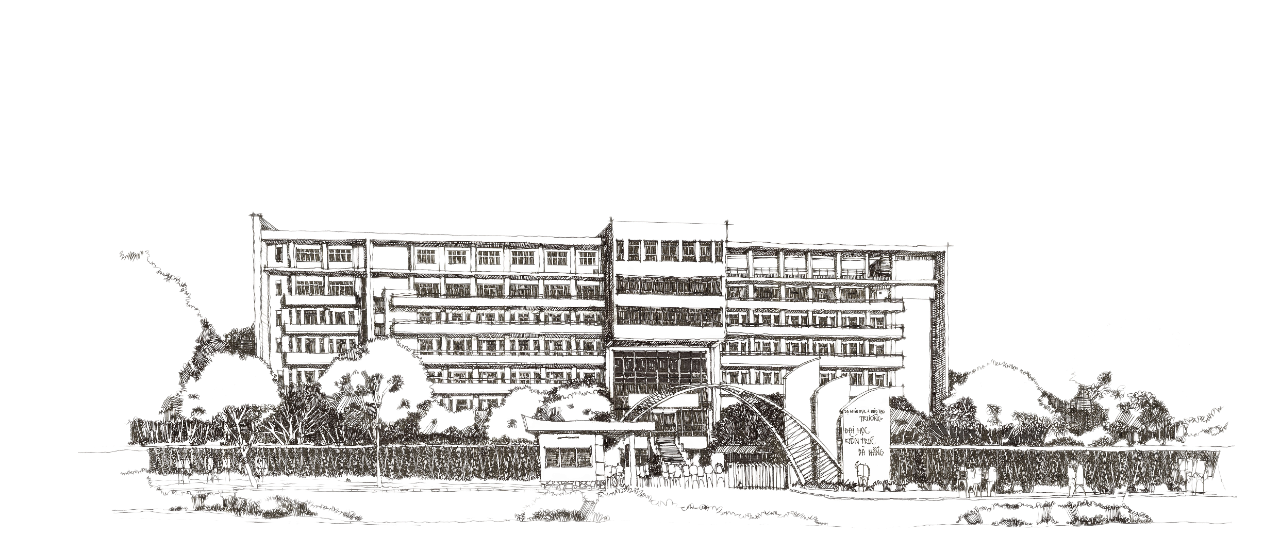
\includegraphics[width=0.7\paperwidth]{dau-campus.png}};
  \node[anchor=north west] at ([xshift=0.55cm, yshift=-0.45cm]current page.north west){
\includegraphics[height=0.9cm]{dau-logo.png}};
  \node[anchor=base, text=daumaroon] at ([yshift=-3.3cm]current page.north){\fontsize{52}{52}\selectfont\bfseries #1};
  \fill[daumaroon] ([yshift=-3.7cm]current page.north west) rectangle ([yshift=-5.15cm]current page.north east);
  \fill[daugold]   ([yshift=-5.15cm]current page.north west) rectangle ([yshift=-5.27cm]current page.north east);
  \node[anchor=center, text=white, align=center, text width=0.9\paperwidth] at ([yshift=-4.42cm]current page.north){\Large\bfseries #2};
\end{tikzpicture}
\end{frame}}}

% ---------- Metadata --------------------------------------------------
\title[Luồng KĐCLGD \, $\cdot$ \, kdcl-v2]{Hệ thống quản lý minh chứng KĐCLGD}
\subtitle{Mô tả luồng nghiệp vụ: đánh giá cơ sở giáo dục và minh chứng chương trình đào tạo}
\author{TS. Đỗ Phúc Hảo, Giám đốc Trung tâm CAIRA}
\institute{Trung tâm CAIRA, Trường Đại học Kiến trúc Đà Nẵng}
\date{\today}

\begin{document}

% ============================ COVER ===================================
{\setbeamertemplate{headline}{}\setbeamertemplate{footline}{}
\begin{frame}[plain]
\begin{tikzpicture}[remember picture, overlay]
  \fill[daunavy] (current page.north west) rectangle (current page.south east);
  \node[anchor=south east, opacity=0.10] at ([xshift=-0.2cm,yshift=0.1cm]current page.south east){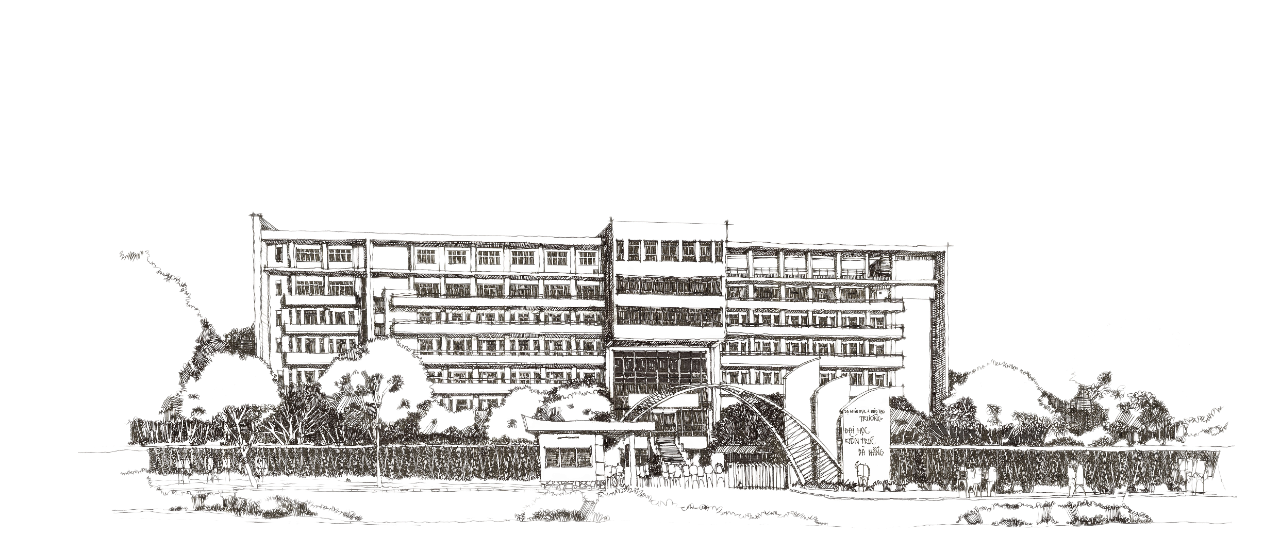
\includegraphics[width=0.55\paperwidth]{dau-campus.png}};
  \fill[daumaroon] ([yshift=-7.05cm]current page.north west) rectangle ([yshift=-7.25cm]current page.north east);
  \fill[daugold]   ([yshift=-7.25cm]current page.north west) rectangle ([yshift=-7.37cm]current page.north east);
  \node[anchor=north west] at ([xshift=0.6cm, yshift=-0.55cm]current page.north west){
\includegraphics[height=1.0cm]{dau-logo.png}};
  \node[anchor=north west, text width=13.6cm, inner sep=0, align=left] at ([xshift=0.6cm, yshift=-1.95cm]current page.north west){%
    \color{white}\raggedright
    {\normalsize\bfseries TRUNG TÂM CAIRA \, $\cdot$ \, TRƯỜNG ĐẠI HỌC KIẾN TRÚC ĐÀ NẴNG}\\[0.42cm]
    {\fontsize{24}{28}\selectfont\bfseries Hệ thống quản lý minh chứng KĐCLGD}\\[0.2cm]
    {\large\color{daugold}\bfseries Luồng đánh giá cơ sở giáo dục \& minh chứng chương trình đào tạo}\\[0.5cm]
    {\small\bfseries Trình bày:} {\small TS. Đỗ Phúc Hảo, Giám đốc Trung tâm CAIRA}\\[0.12cm]
    {\footnotesize\itshape Phần mềm phục vụ tự đánh giá và chuẩn bị đón đoàn kiểm định chất lượng}%
  };
  \node[anchor=north west, text width=13.6cm, inner sep=0, align=left] at ([xshift=0.6cm, yshift=-7.6cm]current page.north west){%
    \color{white!85}\raggedright
    {\footnotesize\itshape ``Số hóa minh chứng \, $\cdot$ \, chuẩn hóa quy trình nộp - duyệt \, $\cdot$ \, sẵn sàng đón đoàn''}\\[0.15cm]
    {\small \today \, $\cdot$ \, Đà Nẵng}%
  };
\end{tikzpicture}
\end{frame}}

% ============================ OUTLINE =================================
\begin{frame}{Nội dung trình bày}
\vspace{0.05cm}
\begin{columns}[T]
\begin{column}{0.5\textwidth}
\textbf{\color{daumaroon}1. Tổng quan hệ thống}
\begin{itemize}\footnotesize
  \item Bối cảnh: hai loại kiểm định
  \item Cơ sở pháp lý và biểu mẫu
  \item Kiến trúc và vai trò người dùng
\end{itemize}
\vspace{0.2cm}
\textbf{\color{daumaroon}2. Luồng đánh giá cơ sở giáo dục}
\begin{itemize}\footnotesize
  \item Năm giai đoạn tự đánh giá
  \item Phân công, nộp và duyệt minh chứng
  \item Vòng đời một minh chứng
  \item Đánh giá tiêu chí, KPI, khảo sát
  \item Báo cáo và đối soát đón đoàn
\end{itemize}
\end{column}
\begin{column}{0.5\textwidth}
\textbf{\color{daumaroon}3. Luồng minh chứng chương trình đào tạo}
\begin{itemize}\footnotesize
  \item Khung chuẩn đầu ra PEO - PLO - CLO
  \item Ma trận ánh xạ và minh chứng
  \item Đo lường CLO lên PLO (AUN-QA)
\end{itemize}
\vspace{0.2cm}
\textbf{\color{daumaroon}4. Tổng hợp và vận hành}
\begin{itemize}\footnotesize
  \item So sánh hai luồng
  \item Triển khai, bảo mật, sao lưu
\end{itemize}
\end{column}
\end{columns}
\vspace{0.12cm}
\begin{keypoint}
Hệ thống hỗ trợ song song \textbf{kiểm định cơ sở giáo dục} (TT26, 15 tiêu chuẩn) và \textbf{kiểm định chương trình đào tạo} (TT04, chuẩn đầu ra), trên cùng một nền tảng quản lý minh chứng.
\end{keypoint}
\end{frame}

% #####################################################################
\section{Tổng quan hệ thống}
\dividerframe{01}{Tổng quan hệ thống}

% ---- Bối cảnh ----
\begin{frame}{Bối cảnh: hai loại kiểm định chất lượng}
\vspace{0.05cm}
\begin{columns}[T]
\begin{column}{0.49\textwidth}
\begin{tcolorbox}[enhanced, colback=lightwarm, colframe=daumaroon, boxrule=0pt, leftrule=3pt, arc=2pt, title=\textbf{Kiểm định CƠ SỞ GIÁO DỤC}, fonttitle=\bfseries\color{white}, coltitle=white, colbacktitle=daumaroon]
\scriptsize
\begin{itemize}
  \item Theo Thông tư 26 (bộ tiêu chuẩn hiện hành)
  \item \textbf{15 tiêu chuẩn / 60 tiêu chí}
  \item Đánh giá toàn trường: quản trị, nhân lực, tài chính, đào tạo, NCKH, bảo đảm chất lượng...
\end{itemize}
\end{tcolorbox}
\end{column}
\begin{column}{0.49\textwidth}
\begin{tcolorbox}[enhanced, colback=lightnavy, colframe=daunavy, boxrule=0pt, leftrule=3pt, arc=2pt, title=\textbf{Kiểm định CHƯƠNG TRÌNH ĐÀO TẠO}, fonttitle=\bfseries\color{white}, coltitle=white, colbacktitle=daunavy]
\scriptsize
\begin{itemize}
  \item Theo Thông tư 04 (tiếp cận AUN-QA)
  \item Trọng tâm \textbf{chuẩn đầu ra}: PEO - PLO - CLO
  \item Minh chứng gắn với chương trình, đề cương, đo lường kết quả học tập
\end{itemize}
\end{tcolorbox}
\end{column}
\end{columns}
\vspace{0.15cm}
\begin{notebox}
\textbf{Thách thức khi đón đoàn:} minh chứng rải rác ở nhiều phòng ban, khó tổng hợp; quy trình nộp - duyệt thủ công, thiếu dấu vết ai nộp, ai xác nhận. \textbf{Phần mềm giải quyết đúng các điểm này.}
\end{notebox}
\end{frame}

% ---- Cơ sở pháp lý ----
\begin{frame}{Cơ sở pháp lý và biểu mẫu áp dụng}
\vspace{0.1cm}
\begin{columns}[T]
\begin{column}{0.49\textwidth}
\begin{tcolorbox}[enhanced, colback=lightwarm, colframe=daumaroon, boxrule=0pt, leftrule=3pt, arc=2pt, title=\textbf{Kiểm định CƠ SỞ GIÁO DỤC}, fonttitle=\bfseries\color{white}, coltitle=white, colbacktitle=daumaroon]
\scriptsize
\begin{itemize}
  \item \textbf{Thông tư 26/2026/TT-BGDĐT} — bộ tiêu chuẩn đánh giá chất lượng cơ sở giáo dục (15 tiêu chuẩn / 60 tiêu chí)
  \item Phụ lục I — hệ thống biểu mẫu tự đánh giá
  \item Phụ lục II — hướng dẫn đánh giá tiêu chí
\end{itemize}
\end{tcolorbox}
\end{column}
\begin{column}{0.49\textwidth}
\begin{tcolorbox}[enhanced, colback=lightnavy, colframe=daunavy, boxrule=0pt, leftrule=3pt, arc=2pt, title=\textbf{Kiểm định CHƯƠNG TRÌNH ĐÀO TẠO}, fonttitle=\bfseries\color{white}, coltitle=white, colbacktitle=daunavy]
\scriptsize
\begin{itemize}
  \item \textbf{Thông tư 04/2025/TT-BGDĐT} — đánh giá chất lượng chương trình đào tạo (tiếp cận AUN-QA)
  \item Hướng dẫn đo chuẩn đầu ra (CLO, PLO) và chuẩn hóa rubric
  \item Tài liệu tham chiếu AUN-QA, ABET
\end{itemize}
\end{tcolorbox}
\end{column}
\end{columns}
\vspace{0.2cm}
\begin{keypoint}
Phần mềm số hóa đúng bộ biểu mẫu ban hành kèm thông tư: \textbf{Biểu 01} thành lập Hội đồng \, $\cdot$ \, \textbf{Biểu 02} kế hoạch TĐG \, $\cdot$ \, \textbf{Biểu 04} đánh giá tiêu chí \, $\cdot$ \, \textbf{Biểu 05} báo cáo TĐG \, $\cdot$ \, \textbf{Biểu 08-11} khảo sát các bên \, $\cdot$ \, \textbf{Biểu 16} số liệu KPI.
\end{keypoint}
\end{frame}

% ---- Kiến trúc [F1] ----
\begin{frame}{Kiến trúc hệ thống}
\vspace{0.1cm}
\begin{center}
\resizebox{0.88\textwidth}{!}{%
\begin{tikzpicture}[node distance=1.1cm]
  \node[kboxn, minimum width=2.7cm] (br) {Trình duyệt\\[-1pt]{\scriptsize\mdseries (đơn vị, P.ĐBCL, đoàn)}};
  \node[kboxm, minimum width=3.2cm, right=1.7cm of br] (app) {Máy chủ ứng dụng\\[-1pt]{\scriptsize\mdseries Node.js + Express}};
  \node[kbox, minimum width=3.0cm, above right=0.35cm and 1.6cm of app] (db) {PostgreSQL\\[-1pt]{\scriptsize\mdseries Dữ liệu (metadata)}};
  \node[kboxg, minimum width=3.0cm, below right=0.35cm and 1.6cm of app] (fs) {Kho tệp \textit{uploads}\\[-1pt]{\scriptsize\mdseries File minh chứng thật}};
  \draw[karrm] (br) -- node[klbl, above]{HTTPS} (app);
  \draw[karr] (app) -- node[klbl, above, sloped]{truy vấn} (db);
  \draw[karr] (app) -- node[klbl, below, sloped]{lưu / tải file} (fs);
  \begin{scope}[on background layer]
    \node[draw=gray300, rounded corners=4pt, fit=(app)(db)(fs), inner sep=10pt, label={[font=\scriptsize\bfseries, text=gray500]below:Đóng gói Docker \, $\cdot$ \, triển khai trên VPS}] {};
  \end{scope}
\end{tikzpicture}}
\end{center}
\vspace{0.15cm}
\begin{columns}[T]
\begin{column}{0.5\textwidth}\footnotesize
\textbf{\color{daumaroon}Metadata trong CSDL:} mã minh chứng, tiêu chí, trạng thái, đơn vị, người nộp/duyệt, đánh giá, KPI, chuẩn đầu ra.
\end{column}
\begin{column}{0.5\textwidth}\footnotesize
\textbf{\color{daumaroon}File trong kho \textit{uploads}:} văn bản thật (PDF, DOCX...); CSDL chỉ lưu tên và đường dẫn. Liên kết ngoài lưu URL (Drive/SharePoint).
\end{column}
\end{columns}
\end{frame}

% ---- Vai trò [F2] ----
\begin{frame}{Vai trò người dùng và không gian làm việc}
\vspace{0.1cm}
\begin{center}
\resizebox{0.94\textwidth}{!}{%
\begin{tikzpicture}[node distance=1.1cm]
  \node[kboxm, text width=3.2cm, minimum height=1.6cm] (ad) {P.ĐBCL — \textit{admin}\\[3pt]{\scriptsize\mdseries Duyệt, trả lại, phân công, quản lý tài khoản}};
  \node[kboxn, text width=3.2cm, minimum height=1.6cm, right=of ad] (un) {Đơn vị — \textit{unit}\\[3pt]{\scriptsize\mdseries Nộp minh chứng cho tiêu chí được giao}};
  \node[kboxg, text width=3.2cm, minimum height=1.6cm, right=of un] (vw) {Lãnh đạo / Đoàn — \textit{viewer}\\[3pt]{\scriptsize\mdseries Xem dashboard, đối soát tiêu chí}};
\end{tikzpicture}}
\end{center}
\vspace{0.25cm}
\begin{columns}[T]
\begin{column}{0.62\textwidth}
\begin{keypoint}
Mỗi \textbf{đợt kiểm định} là một ``không gian làm việc'' (workspace) riêng: chọn loại \textbf{CSGD} hoặc \textbf{CTĐT}. Dữ liệu các đợt tách biệt hoàn toàn, có thể chạy song song nhiều đợt.
\end{keypoint}
\end{column}
\begin{column}{0.36\textwidth}
\begin{notebox}
Đăng nhập theo vai bằng mật khẩu băm; mọi thao tác nộp/duyệt lưu \textbf{tên người thật} và thời gian, tạo dấu vết kiểm toán.
\end{notebox}
\end{column}
\end{columns}
\end{frame}

% #####################################################################
\section{Luồng đánh giá cơ sở giáo dục}
\dividerframe{02}{Luồng đánh giá\\[2pt] cơ sở giáo dục}

% ---- Tổng quan 5 GĐ [F3] ----
\begin{frame}{Quy trình tự đánh giá: năm giai đoạn}
\vspace{0.35cm}
\begin{center}
\resizebox{0.99\textwidth}{!}{%
\begin{tikzpicture}[node distance=0.55cm]
  \node[kboxm, minimum width=2.7cm, minimum height=1.35cm] (g1) {1. Thành lập\\ Hội đồng TĐG\\[1pt]{\scriptsize\mdseries Kế hoạch 24 tuần}};
  \node[kboxn, minimum width=2.7cm, minimum height=1.35cm, right=0.75cm of g1] (g2) {2. Thu thập\\ minh chứng\\[1pt]{\scriptsize\mdseries Nộp - duyệt theo đơn vị}};
  \node[kboxn, minimum width=2.7cm, minimum height=1.35cm, right=0.75cm of g2] (g3) {3. Đánh giá\\ 60 tiêu chí\\[1pt]{\scriptsize\mdseries KPI, khảo sát}};
  \node[kboxn, minimum width=2.7cm, minimum height=1.35cm, right=0.75cm of g3] (g4) {4. Viết\\ Báo cáo TĐG\\[1pt]{\scriptsize\mdseries Biểu 05}};
  \node[kboxg, minimum width=2.7cm, minimum height=1.35cm, right=0.75cm of g4] (g5) {5. Thẩm định\\ \& đón đoàn\\[1pt]{\scriptsize\mdseries Đối soát độ phủ}};
  \draw[karrm] (g1) -- (g2); \draw[karrm] (g2) -- (g3); \draw[karrm] (g3) -- (g4); \draw[karrm] (g4) -- (g5);
\end{tikzpicture}}
\end{center}
\vspace{0.3cm}
\begin{notebox}
Phần mềm số hóa cả năm giai đoạn. Module \textbf{Tiến độ TĐG} theo dõi kế hoạch 24 tuần; ba slide tiếp theo đi sâu vào giai đoạn cốt lõi: \textbf{thu thập, nộp và duyệt minh chứng theo đơn vị}.
\end{notebox}
\end{frame}

% ---- GĐ1 ----
\begin{frame}{Giai đoạn 1: Thành lập Hội đồng và kế hoạch}
\vspace{0.15cm}
\begin{columns}[T]
\begin{column}{0.56\textwidth}\footnotesize
\textbf{\color{daumaroon}Module Tiến độ TĐG} quản lý kế hoạch tự đánh giá chuẩn \textbf{24 tuần / 5 pha}:
\begin{itemize}
  \item Ra quyết định thành lập Hội đồng, phân công nhóm chuyên trách
  \item Sinh sẵn danh sách công việc theo mẫu, gắn tuần bắt đầu - kết thúc
  \item Theo dõi trạng thái: \textit{chưa làm / đang làm / hoàn thành / trễ hạn}
\end{itemize}
\end{column}
\begin{column}{0.42\textwidth}
\begin{tcolorbox}[enhanced, colback=gray100, colframe=daumaroon, boxrule=0pt, leftrule=3pt, arc=2pt, fontupper=\scriptsize]
\textbf{\color{daumaroon}Kết quả:} mỗi công việc có người phụ trách và mốc thời gian, giúp lãnh đạo nhìn nhanh tiến độ toàn đợt kiểm định và các đầu việc đang trễ.
\end{tcolorbox}
\end{column}
\end{columns}
\end{frame}

% ---- GĐ2 phân công [F4] ----
\begin{frame}{Giai đoạn 2a: Phân công tiêu chí cho đơn vị}
\vspace{0.1cm}
\begin{center}
\resizebox{!}{3.6cm}{%
\begin{tikzpicture}[node distance=0.35cm and 0.5cm]
  \node[kboxm, minimum width=2.9cm] (u1) {Phòng Đào tạo};
  \node[kboxm, minimum width=2.9cm, below=of u1] (u2) {Khoa CNTT};
  \node[kboxm, minimum width=2.9cm, below=of u2] (u3) {Phòng TC-HC};
  \node[kboxm, minimum width=2.9cm, below=of u3] (u4) {P.ĐBCL};
  \foreach \r/\y in {u1/0, u2/-1.15, u3/-2.3, u4/-3.45} {}
  \node[kbox, minimum width=1.5cm, right=1.7cm of u1] (t1) {TC 6.1};
  \node[kbox, minimum width=1.5cm, right=0.35cm of t1] (t2) {TC 6.2};
  \node[kbox, minimum width=1.5cm, right=0.35cm of t2] (t3) {TC 6.4};
  \node[kbox, minimum width=1.5cm, right=1.7cm of u2] (t4) {TC 6.3};
  \node[kbox, minimum width=1.5cm, right=0.35cm of t4] (t5) {TC 7.4};
  \node[kbox, minimum width=1.5cm, right=1.7cm of u3] (t6) {TC 3.1};
  \node[kbox, minimum width=1.5cm, right=0.35cm of t6] (t7) {TC 3.2};
  \node[kbox, minimum width=1.5cm, right=1.7cm of u4] (t8) {TC 9.1};
  \node[kbox, minimum width=1.5cm, right=0.35cm of t8] (t9) {TC 10.1};
  \draw[karr](u1)--(t1); \draw[karr](u2)--(t4); \draw[karr](u3)--(t6); \draw[karr](u4)--(t8);
\end{tikzpicture}}
\end{center}
\vspace{0.1cm}
\begin{keypoint}
P.ĐBCL gán mỗi tiêu chí cho đơn vị chịu trách nhiệm. Nhờ đó mỗi phòng/khoa \textbf{chỉ thấy phần việc của mình} ở Cổng đơn vị, tránh chồng chéo và bỏ sót.
\end{keypoint}
\end{frame}

% ---- Cổng đơn vị ----
\begin{frame}{Giai đoạn 2b: Cổng đơn vị nộp minh chứng}
\vspace{0.15cm}
\begin{columns}[T]
\begin{column}{0.54\textwidth}\footnotesize
Đơn vị đăng nhập, vào \textbf{Cổng đơn vị}, thấy các tiêu chí được giao và tải minh chứng lên theo \textbf{hai hình thức}:
\begin{itemize}
  \item \textbf{Tải tệp} trực tiếp lên máy chủ (PDF, DOCX, ảnh...)
  \item \textbf{Dán liên kết} Google Drive / SharePoint
\end{itemize}
Hệ thống tự sinh mã minh chứng chuẩn \texttt{Hn.ab.cd.ef} và đặt trạng thái \textbf{chờ duyệt}.
\end{column}
\begin{column}{0.44\textwidth}
\begin{tcolorbox}[enhanced, colback=lightgold, colframe=daugold!80!black, boxrule=0pt, leftrule=3pt, arc=2pt, fontupper=\scriptsize]
\textbf{Linh hoạt theo thói quen:} phòng nào quen Drive thì dán liên kết; phòng khác tải tệp trực tiếp. Cùng một quy trình duyệt cho cả hai.
\end{tcolorbox}
\vspace{0.15cm}
\begin{tcolorbox}[enhanced, colback=lightgreen, colframe=okgreen, boxrule=0pt, leftrule=3pt, arc=2pt, fontupper=\scriptsize]
Đơn vị theo dõi được trạng thái từng minh chứng và lý do nếu bị trả lại.
\end{tcolorbox}
\end{column}
\end{columns}
\end{frame}

% ---- Bàn duyệt [F5] swimlane ----
\begin{frame}{Giai đoạn 2c: Bàn duyệt của P.ĐBCL}
\vspace{0.05cm}
\begin{center}
\resizebox{!}{3.4cm}{%
\begin{tikzpicture}
  % nhãn lane
  \node[font=\bfseries\footnotesize, text=daunavy,   anchor=east] (lu) at (1.1, 0)    {ĐƠN VỊ};
  \node[font=\bfseries\footnotesize, text=daumaroon, anchor=east] (lp) at (1.1, -2.3) {P.ĐBCL};
  % lane trên (đơn vị)
  \node[kboxn,     minimum width=2.6cm, anchor=west] (up)   at (1.5, 0)    {Tải minh chứng};
  \node[waitstate, minimum width=2.4cm, anchor=west] (wait) at (5.4, 0)    {Chờ duyệt};
  % lane dưới (P.ĐBCL)
  \node[kboxm,     minimum width=2.6cm, anchor=west] (rev)  at (1.5, -2.3) {Xem, mở tệp};
  \node[okstate,   minimum width=2.4cm, anchor=west] (ok)   at (5.4, -1.6) {Đã xác nhận};
  \node[backstate, minimum width=2.6cm, anchor=west] (back) at (5.4, -3.0) {Trả lại (kèm lý do)};
  % luồng
  \draw[karrm] (up) -- (wait);
  \draw[karr]  (wait.south) -- ([yshift=-0.7cm]wait.south) -| (rev.north);
  \draw[karrm] (rev.east) -- (ok.west);
  \draw[karrm] (rev.east) -- (back.west);
  \draw[karr]  (back.south) -- ([yshift=-0.55cm]back.south)
               -| ($(lu.east)!0.5!(up.west)$) |- (up.west);
  \node[klbl] at ([yshift=-0.55cm]back.south -| up) {nộp bản thay thế};
\end{tikzpicture}}
\end{center}
\vspace{0.15cm}
\begin{keypoint}
P.ĐBCL duyệt tập trung: \textbf{xác nhận} nếu đạt, hoặc \textbf{trả lại kèm lý do} để đơn vị bổ sung. Chỉ minh chứng \textbf{đã xác nhận} mới được tính khi đối soát và đón đoàn.
\end{keypoint}
\end{frame}

% ---- Vòng đời MC [F6] state machine ----
\begin{frame}{Vòng đời một minh chứng}
\vspace{0.35cm}
\begin{center}
\resizebox{0.96\textwidth}{!}{%
\begin{tikzpicture}[node distance=1.5cm]
  \node[nonestate, minimum width=2.3cm] (s0) {Chưa nộp};
  \node[waitstate, minimum width=2.3cm, right=of s0] (s1) {Chờ duyệt};
  \node[okstate,   minimum width=2.3cm, right=of s1] (s2) {Đã xác nhận};
  \node[backstate, minimum width=2.3cm, below=1.4cm of s1] (s3) {Bị trả lại};
  \draw[karrm] (s0) -- node[klbl, above]{đơn vị nộp} (s1);
  \draw[karrm] (s1) -- node[klbl, above]{P.ĐBCL xác nhận} (s2);
  \draw[karrm] ([xshift=-4mm]s1.south) -- node[klbl, left]{trả lại} ([xshift=-4mm]s3.north);
  \draw[karr]  ([xshift=4mm]s3.north)  -- node[klbl, right]{nộp lại} ([xshift=4mm]s1.south);
\end{tikzpicture}}
\end{center}
\vspace{0.2cm}
\begin{notebox}
Mỗi lần chuyển trạng thái đều lưu \textbf{người thực hiện} và \textbf{thời gian}. ``Bị trả lại'' luôn kèm \textbf{lý do} để đơn vị biết cần sửa gì. Đây chính là dấu vết kiểm toán đoàn thường hỏi.
\end{notebox}
\end{frame}

% ---- Đánh giá + KPI + khảo sát ----
\begin{frame}{Giai đoạn 3: Đánh giá tiêu chí, KPI, khảo sát}
\vspace{0.1cm}
\begin{columns}[T]
\begin{column}{0.34\textwidth}
\begin{tcolorbox}[enhanced, colback=lightwarm, colframe=daumaroon, boxrule=0pt, leftrule=3pt, arc=2pt, title=Đánh giá 60 tiêu chí, fonttitle=\scriptsize\bfseries\color{white}, coltitle=white, colbacktitle=daumaroon, fontupper=\scriptsize]
Mỗi tiêu chí (Biểu 04): hiện trạng, điểm mạnh, tồn tại, kế hoạch; kết quả \textbf{Đạt / Không đạt}; nháp hay đã duyệt.
\end{tcolorbox}
\end{column}
\begin{column}{0.32\textwidth}
\begin{tcolorbox}[enhanced, colback=lightnavy, colframe=daunavy, boxrule=0pt, leftrule=3pt, arc=2pt, title=KPI (Biểu 16), fonttitle=\scriptsize\bfseries\color{white}, coltitle=white, colbacktitle=daunavy, fontupper=\scriptsize]
Số liệu theo \textbf{năm học}: đội ngũ, người học, tốt nghiệp, việc làm, công bố khoa học... để so sánh xu hướng.
\end{tcolorbox}
\end{column}
\begin{column}{0.32\textwidth}
\begin{tcolorbox}[enhanced, colback=lightgold, colframe=daugold!80!black, boxrule=0pt, leftrule=3pt, arc=2pt, title=Khảo sát (Biểu 08-11), fonttitle=\scriptsize\bfseries\color{daunavy}, coltitle=daunavy, colbacktitle=daugold, fontupper=\scriptsize]
Cán bộ, người học, nhà tuyển dụng, cựu sinh viên; thang Likert; \textbf{liên kết công khai} theo mã, tự tổng hợp.
\end{tcolorbox}
\end{column}
\end{columns}
\vspace{0.3cm}
\begin{keypoint}
Ba nguồn dữ liệu (đánh giá định tính, KPI định lượng, khảo sát các bên) bổ trợ nhau, làm cơ sở viết Báo cáo tự đánh giá và minh chứng cho từng tiêu chí.
\end{keypoint}
\end{frame}

% ---- Báo cáo + đối soát [F7] ----
\begin{frame}{Giai đoạn 4-5: Báo cáo và đối soát đón đoàn}
\vspace{0.1cm}
\begin{columns}[T]
\begin{column}{0.42\textwidth}\footnotesize
\textbf{\color{daumaroon}Báo cáo TĐG (Biểu 05)} tổng hợp cơ sở pháp lý, quá trình, kết quả 15 tiêu chuẩn và kế hoạch cải tiến.
\vspace{0.2cm}

\textbf{\color{daumaroon}Đối soát đón đoàn:} mỗi tiêu chí hiển thị các minh chứng \textbf{đã xác nhận}; heatmap cho biết độ phủ toàn cục.
\end{column}
\begin{column}{0.56\textwidth}
\begin{center}
\resizebox{0.99\textwidth}{!}{%
\begin{tikzpicture}[x=0.62cm, y=0.62cm]
  \foreach \i/\lab in {0/TC1,1/TC2,2/TC3,3/TC4,4/TC5,5/TC6,6/TC7,7/TC8,8/TC9,9/TC10,10/TC11,11/TC12,12/TC13,13/TC14,14/TC15}
    \node[font=\tiny, text=gray500] at (\i+0.5, 5.4) {\lab};
  % 4 hàng tiêu chí minh hoạ; mẫu màu tất định (xanh nhiều, vàng/xám xen kẽ)
  \foreach \r in {0,...,3} {
    \foreach \i in {0,...,14} {
      \pgfmathtruncatemacro{\v}{mod(\i*3+\r*5+\i*\i, 5)}
      \ifcase\v \def\fc{okgreen}\or\def\fc{okgreen}\or\def\fc{daugold}\or\def\fc{okgreen}\or\def\fc{gray300}\fi
      \fill[\fc] (\i, 5-\r) rectangle ++(0.9,0.9);
    }
  }
  \node[okstate, font=\tiny, minimum width=1.6cm, minimum height=0.5cm] at (2.2,-0.4){Đủ};
  \node[waitstate, font=\tiny, minimum width=1.8cm, minimum height=0.5cm] at (6.4,-0.4){Đang duyệt};
  \node[nonestate, font=\tiny, minimum width=1.6cm, minimum height=0.5cm] at (10.6,-0.4){Thiếu};
\end{tikzpicture}}
\end{center}
\end{column}
\end{columns}
\vspace{0.1cm}
\begin{notebox}
\textbf{Dashboard} cho lãnh đạo: tiến độ nộp/duyệt theo đơn vị và độ phủ minh chứng theo tiêu chí, giúp biết \textbf{còn thiếu chỗ nào} trước khi đón đoàn.
\end{notebox}
\end{frame}

% ---- Luồng thực hiện chi tiết CSGD ----
\begin{frame}{Luồng thực hiện chi tiết trên phần mềm (CSGD)}
\vspace{0.15cm}
\begin{center}
\resizebox{0.98\textwidth}{!}{%
\begin{tikzpicture}[node distance=0.65cm]
  \node[stepcard] (c1) {\textbf{1. Tạo đợt kiểm định (CSGD) và cấp tài khoản đơn vị}\\[2pt]{\tiny\itshape P.ĐBCL}};
  \node[stepcard, right=of c1] (c2) {\textbf{2. Phân công tiêu chí cho từng đơn vị phụ trách}\\[2pt]{\tiny\itshape P.ĐBCL}};
  \node[stepcard, right=of c2] (c3) {\textbf{3. Nộp minh chứng: tải tệp hoặc dán liên kết Drive}\\[2pt]{\tiny\itshape Đơn vị · Cổng đơn vị}};
  \node[stepcard, below=of c3] (c4) {\textbf{4. Xác nhận hoặc trả lại minh chứng kèm lý do}\\[2pt]{\tiny\itshape P.ĐBCL · Bàn duyệt}};
  \node[stepcard, left=of c4] (c5) {\textbf{5. Đánh giá 60 tiêu chí, nhập KPI, mở khảo sát}\\[2pt]{\tiny\itshape Nhóm chuyên trách}};
  \node[stepcard, left=of c5] (c6) {\textbf{6. Viết báo cáo, đối soát độ phủ, sẵn sàng đón đoàn}\\[2pt]{\tiny\itshape Hội đồng TĐG}};
  \draw[karrm] (c1)--(c2); \draw[karrm] (c2)--(c3); \draw[karrm] (c3)--(c4); \draw[karrm] (c4)--(c5); \draw[karrm] (c5)--(c6);
\end{tikzpicture}}
\end{center}
\vspace{0.1cm}
\begin{notebox}
Toàn bộ sáu bước thực hiện ngay trên phần mềm, mỗi bước ứng với một module. Vai trò phân định rõ: \textbf{P.ĐBCL} điều phối và duyệt, \textbf{đơn vị} nộp minh chứng, \textbf{nhóm chuyên trách} đánh giá và viết báo cáo.
\end{notebox}
\end{frame}

% #####################################################################
\section{Luồng minh chứng chương trình đào tạo}
\dividerframe{03}{Luồng minh chứng\\[2pt] chương trình đào tạo}

% ---- CTĐT khác CSGD ----
\begin{frame}{Chương trình đào tạo khác gì cơ sở giáo dục?}
\vspace{0.15cm}
\begin{columns}[T]
\begin{column}{0.5\textwidth}\footnotesize
\textbf{\color{daumaroon}Giữ nguyên} toàn bộ quy trình đã trình bày:
\begin{itemize}
  \item Phân công tiêu chí cho đơn vị
  \item Nộp - duyệt minh chứng theo đơn vị
  \item Đánh giá tiêu chí, khảo sát, báo cáo
\end{itemize}
\end{column}
\begin{column}{0.5\textwidth}\footnotesize
\textbf{\color{daunavy}Bổ sung} phần đặc thù chương trình:
\begin{itemize}
  \item Khung \textbf{chuẩn đầu ra}: PEO - PLO - CLO
  \item Ma trận ánh xạ học phần lên chuẩn đầu ra
  \item \textbf{Đo lường} kết quả học tập (CLO lên PLO)
\end{itemize}
\end{column}
\end{columns}
\vspace{0.15cm}
\begin{keypoint}
Minh chứng của chương trình đào tạo gắn chặt với chuẩn đầu ra: chương trình, đề cương học phần, rubric, bảng ánh xạ và kết quả đo lường CLO đều là minh chứng phục vụ đánh giá.
\end{keypoint}
\end{frame}

% ---- Khung CĐR [F8] ----
\begin{frame}{Khung chuẩn đầu ra: PEO - PLO - CLO}
\vspace{0.2cm}
\begin{center}
\resizebox{0.93\textwidth}{!}{%
\begin{tikzpicture}[x=1cm, y=1cm]
  \node[kboxm, text width=7.5cm, minimum height=0.72cm] (peo) at (5.75,1.75) {PEO \, — \, Mục tiêu giáo dục của chương trình};
  \foreach \i in {1,...,4} \node[kboxn, minimum width=1.95cm, minimum height=0.72cm] (p\i) at (\i*2.3,0) {PLO\i};
  \foreach \i in {1,...,4} \node[kbox, minimum width=1.95cm, minimum height=0.72cm] (c\i) at (\i*2.3,-1.75) {CLO của HP};
  \foreach \i in {1,...,4}{\draw[karrm] (peo) -- (p\i); \draw[karr] (p\i) -- (c\i);}
  \node[font=\scriptsize\bfseries, text=gray500, anchor=east] at (0.5,1.75){Mục tiêu};
  \node[font=\scriptsize\bfseries, text=gray500, anchor=east] at (0.5,0){CĐR chương trình};
  \node[font=\scriptsize\bfseries, text=gray500, anchor=east] at (0.5,-1.75){CĐR học phần};
\end{tikzpicture}}
\end{center}
\vspace{0.1cm}
\begin{notebox}
\textbf{PEO} (mục tiêu, 3-5 năm sau tốt nghiệp) $\rightarrow$ \textbf{PLO} (chuẩn đầu ra chương trình, 6-8 mục) $\rightarrow$ \textbf{CLO} (chuẩn đầu ra từng học phần). Học phần đóng góp CLO, CLO ánh xạ lên PLO theo trọng số.
\end{notebox}
\end{frame}

% ---- Ma trận ánh xạ [F9] ----
\begin{frame}{Ma trận ánh xạ học phần lên chuẩn đầu ra}
\vspace{0.2cm}
\begin{columns}[T]
\begin{column}{0.62\textwidth}
\begin{center}
\resizebox{0.99\textwidth}{!}{%
\begin{tikzpicture}[x=1.5cm, y=0.95cm]
  \foreach \j/\p in {1/PLO1,2/PLO2,3/PLO3,4/PLO4,5/PLO5}
    \node[font=\footnotesize\bfseries, text=daunavy] at (\j,3){\p};
  \foreach \i/\c in {1/IT101,2/IT201,3/IT301}
    \node[font=\footnotesize\bfseries, text=daumaroon, anchor=east] at (0.55,3-\i){\c};
  \foreach \i/\j/\lv in {1/1/I,1/2/I, 2/1/R,2/3/I, 3/2/R,3/3/R,3/5/I}
    \node[draw=daugold!80!black, fill=lightgold, rounded corners=2pt, minimum size=0.62cm, font=\footnotesize\bfseries, text=daumaroon] at (\j,3-\i){\lv};
\end{tikzpicture}}
\end{center}
\end{column}
\begin{column}{0.36\textwidth}\footnotesize
Mỗi ô ghi mức đóng góp của học phần cho chuẩn đầu ra:
\begin{itemize}
  \item \textbf{I} — Introduce (giới thiệu)
  \item \textbf{R} — Reinforce (củng cố)
  \item \textbf{M} — Master (thành thạo)
\end{itemize}
\vspace{0.1cm}
\begin{notebox}
Ma trận này là một minh chứng quan trọng, cho thấy chương trình phủ đủ các chuẩn đầu ra.
\end{notebox}
\end{column}
\end{columns}
\end{frame}

% ---- Minh chứng chương trình ----
\begin{frame}{Minh chứng đặc thù của chương trình đào tạo}
\vspace{0.2cm}
\begin{columns}[T]
\begin{column}{0.33\textwidth}
\begin{tcolorbox}[enhanced, colback=lightwarm, colframe=daumaroon, boxrule=0pt, leftrule=3pt, arc=2pt, title=Thiết kế chương trình, fonttitle=\scriptsize\bfseries\color{white}, coltitle=white, colbacktitle=daumaroon, fontupper=\scriptsize]
Chương trình đào tạo bản ban hành, ma trận chuẩn đầu ra và học phần (curriculum map).
\end{tcolorbox}
\end{column}
\begin{column}{0.33\textwidth}
\begin{tcolorbox}[enhanced, colback=lightnavy, colframe=daunavy, boxrule=0pt, leftrule=3pt, arc=2pt, title=Tổ chức dạy học, fonttitle=\scriptsize\bfseries\color{white}, coltitle=white, colbacktitle=daunavy, fontupper=\scriptsize]
Đề cương chi tiết học phần, rubric đánh giá chuẩn đầu ra học phần (CLO).
\end{tcolorbox}
\end{column}
\begin{column}{0.33\textwidth}
\begin{tcolorbox}[enhanced, colback=lightgold, colframe=daugold!80!black, boxrule=0pt, leftrule=3pt, arc=2pt, title=Kết quả đo lường, fonttitle=\scriptsize\bfseries\color{daunavy}, coltitle=daunavy, colbacktitle=daugold, fontupper=\scriptsize]
Bảng điểm, kết quả đo CLO và PLO, báo cáo cải tiến chương trình.
\end{tcolorbox}
\end{column}
\end{columns}
\vspace{0.3cm}
\begin{keypoint}
Tất cả minh chứng trên vẫn đi qua đúng quy trình \textbf{nộp - duyệt theo đơn vị} như luồng cơ sở giáo dục: khoa/bộ môn nộp, P.ĐBCL xác nhận, đối soát theo tiêu chí khi đón đoàn.
\end{keypoint}
\end{frame}

% ---- Đo lường CLO->PLO [F10] ----
\begin{frame}{Đo lường kết quả học tập: CLO lên PLO}
\vspace{0.35cm}
\begin{center}
\resizebox{0.99\textwidth}{!}{%
\begin{tikzpicture}[node distance=0.55cm]
  \node[kboxn, text width=2.4cm, minimum height=1.25cm] (b1) {Điểm sinh viên theo từng bài};
  \node[kboxn, text width=2.4cm, minimum height=1.25cm, right=0.7cm of b1] (b2) {Điểm CLO (theo trọng số)};
  \node[kboxn, text width=2.4cm, minimum height=1.25cm, right=0.7cm of b2] (b3) {Tỉ lệ sinh viên đạt CLO};
  \node[kboxm, text width=2.4cm, minimum height=1.25cm, right=0.7cm of b3] (b4) {Điểm PLO (theo trọng số CLO)};
  \node[kboxg, text width=2.4cm, minimum height=1.25cm, right=0.7cm of b4] (b5) {Phân loại 4 mức AUN-QA};
  \draw[karrm] (b1) -- (b2); \draw[karrm] (b2) -- (b3); \draw[karrm] (b3) -- (b4); \draw[karrm] (b4) -- (b5);
\end{tikzpicture}}
\end{center}
\vspace{0.25cm}
\begin{notebox}
Bốn mức AUN-QA theo tỉ lệ đạt: \textbf{$\geq$75\%} đạt hoàn toàn \, $\cdot$ \, \textbf{$\geq$50\%} đạt \, $\cdot$ \, \textbf{$\geq$25\%} chưa đạt \, $\cdot$ \, \textbf{$<$25\%} chưa đạt hoàn toàn. Hệ thống tính tự động từ điểm nhập vào, xuất kết quả theo học phần và tổng hợp toàn chương trình.
\end{notebox}
\end{frame}

% ---- Luồng thực hiện chi tiết CTĐT ----
\begin{frame}{Luồng thực hiện chi tiết trên phần mềm (CTĐT)}
\vspace{0.15cm}
\begin{center}
\resizebox{0.98\textwidth}{!}{%
\begin{tikzpicture}[node distance=0.65cm]
  \node[stepcard] (d1) {\textbf{1. Tạo đợt kiểm định chương trình (CTĐT) cho ngành}\\[2pt]{\tiny\itshape P.ĐBCL}};
  \node[stepcard, right=of d1] (d2) {\textbf{2. Khai báo khung chuẩn đầu ra: PEO, PLO, học phần, CLO}\\[2pt]{\tiny\itshape Khoa · Bộ môn}};
  \node[stepcard, right=of d2] (d3) {\textbf{3. Lập ma trận ánh xạ học phần lên PLO (I/R/M) và CLO lên PLO}\\[2pt]{\tiny\itshape Khoa}};
  \node[stepcard, below=of d3] (d4) {\textbf{4. Tạo rubric và kế hoạch đo CLO: bài đánh giá, danh sách SV}\\[2pt]{\tiny\itshape Giảng viên}};
  \node[stepcard, left=of d4] (d5) {\textbf{5. Nhập điểm; hệ thống tự tính CLO\% và PLO\% (AUN-QA)}\\[2pt]{\tiny\itshape Giảng viên · hệ thống}};
  \node[stepcard, left=of d5] (d6) {\textbf{6. Nộp/duyệt minh chứng chương trình và viết báo cáo}\\[2pt]{\tiny\itshape Đơn vị · P.ĐBCL}};
  \draw[karrm] (d1)--(d2); \draw[karrm] (d2)--(d3); \draw[karrm] (d3)--(d4); \draw[karrm] (d4)--(d5); \draw[karrm] (d5)--(d6);
\end{tikzpicture}}
\end{center}
\vspace{0.1cm}
\begin{notebox}
Điểm khác biệt nằm ở bước 2 đến 5: xây dựng khung chuẩn đầu ra, ánh xạ và \textbf{đo lường tự động} CLO lên PLO. Bước nộp - duyệt minh chứng (bước 6) dùng chung quy trình với luồng cơ sở giáo dục.
\end{notebox}
\end{frame}

% #####################################################################
\section{Tổng hợp và vận hành}
\dividerframe{04}{Tổng hợp\\[2pt] và vận hành}

% ---- So sánh 2 luồng ----
\begin{frame}{So sánh hai luồng}
\vspace{0.1cm}
{\scriptsize
\begin{tabularx}{\textwidth}{@{}p{3.2cm}XX@{}}
\toprule
\textbf{Khía cạnh} & \textbf{\color{daumaroon}Cơ sở giáo dục (CSGD)} & \textbf{\color{daunavy}Chương trình đào tạo (CTĐT)} \\
\midrule
Cơ sở pháp lý & Thông tư 26 & Thông tư 04 (AUN-QA) \\
Phạm vi & Toàn trường, 15 tiêu chuẩn / 60 tiêu chí & Một chương trình, theo chuẩn đầu ra \\
Nộp - duyệt minh chứng & \multicolumn{2}{c}{\cellcolor{lightwarm}\textbf{Dùng chung} một quy trình theo đơn vị} \\
Đặc thù & KPI toàn trường, khảo sát các bên & Khung PEO-PLO-CLO, đo lường CLO lên PLO \\
Kết quả chính & Báo cáo tự đánh giá 15 tiêu chuẩn & Mức đạt chuẩn đầu ra (4 mức AUN-QA) \\
\bottomrule
\end{tabularx}}
\vspace{0.12cm}
\begin{keypoint}
Hai luồng chia sẻ chung phần lõi (không gian làm việc, đơn vị, nộp - duyệt minh chứng, dashboard); chỉ khác ở phần đặc thù. Nhờ đó vận hành nhất quán, dễ đào tạo người dùng.
\end{keypoint}
\end{frame}

% ---- Điểm nổi bật ----
\begin{frame}{Điểm nổi bật của hệ thống}
\vspace{0.15cm}
\begin{columns}[T]
\begin{column}{0.5\textwidth}
\begin{tcolorbox}[enhanced, colback=lightwarm, colframe=daumaroon, boxrule=0pt, leftrule=3pt, arc=2pt, fontupper=\footnotesize]
\textbf{\color{daumaroon}Quy trình có kiểm soát}
\begin{itemize}\scriptsize
  \item Nộp - duyệt theo đơn vị, có xác nhận và trả lại kèm lý do
  \item Dấu vết kiểm toán: ai nộp, ai duyệt, khi nào
\end{itemize}
\end{tcolorbox}
\vspace{0.1cm}
\begin{tcolorbox}[enhanced, colback=lightnavy, colframe=daunavy, boxrule=0pt, leftrule=3pt, arc=2pt, fontupper=\footnotesize]
\textbf{\color{daunavy}Sẵn sàng đón đoàn}
\begin{itemize}\scriptsize
  \item Đối soát minh chứng theo từng tiêu chí
  \item Dashboard độ phủ, biết ngay còn thiếu chỗ nào
\end{itemize}
\end{tcolorbox}
\end{column}
\begin{column}{0.5\textwidth}
\begin{tcolorbox}[enhanced, colback=lightgreen, colframe=okgreen, boxrule=0pt, leftrule=3pt, arc=2pt, fontupper=\footnotesize]
\textbf{\color{okgreen}Linh hoạt và mở rộng}
\begin{itemize}\scriptsize
  \item Nhiều đợt kiểm định song song (CSGD và CTĐT)
  \item Lưu tệp trực tiếp hoặc liên kết Drive
  \item Đo lường chuẩn đầu ra theo AUN-QA
\end{itemize}
\end{tcolorbox}
\vspace{0.1cm}
\begin{tcolorbox}[enhanced, colback=lightgold, colframe=daugold!80!black, boxrule=0pt, leftrule=3pt, arc=2pt, fontupper=\footnotesize]
\textbf{\color{daunavy}Chủ động về dữ liệu}
\begin{itemize}\scriptsize
  \item Dữ liệu và tệp nằm trên máy chủ của trường
  \item Đóng gói Docker, sao lưu định kỳ
\end{itemize}
\end{tcolorbox}
\end{column}
\end{columns}
\end{frame}

% ---- Triển khai [F-deploy] ----
\begin{frame}{Triển khai, bảo mật và sao lưu}
\vspace{0.15cm}
\begin{center}
\resizebox{0.97\textwidth}{!}{%
\begin{tikzpicture}[node distance=1.0cm]
  \node[kboxn, text width=2.0cm, minimum height=1.0cm] (net) {Internet\\{\scriptsize\mdseries người dùng}};
  \node[kboxg, text width=2.6cm, minimum height=1.0cm, right=1.1cm of net] (rp) {Reverse proxy\\{\scriptsize\mdseries HTTPS, tên miền}};
  \node[kboxm, text width=2.6cm, minimum height=1.0cm, right=1.1cm of rp] (app) {Ứng dụng\\{\scriptsize\mdseries container Docker}};
  \node[kbox, text width=2.6cm, minimum height=1.0cm, right=1.1cm of app] (data) {Dữ liệu bền\\{\scriptsize\mdseries Postgres + tệp}};
  \draw[karrm] (net) -- node[klbl, above]{443} (rp);
  \draw[karrm] (rp) -- (app);
  \draw[karr] (app) -- (data);
  \node[kboxg, text width=2.6cm, minimum height=0.75cm, below=0.8cm of data] (bk) {Sao lưu ZIP};
  \draw[karr] (data) -- node[klbl, right]{định kỳ} (bk);
\end{tikzpicture}}
\end{center}
\vspace{0.1cm}
\begin{columns}[T]
\begin{column}{0.5\textwidth}\scriptsize
\textbf{\color{daumaroon}Bảo mật:} cổng ứng dụng và cơ sở dữ liệu chỉ mở nội bộ; ra ngoài chỉ qua reverse proxy có HTTPS. Đổi mật khẩu quản trị và cơ sở dữ liệu khi chạy thật.
\end{column}
\begin{column}{0.5\textwidth}\scriptsize
\textbf{\color{daumaroon}Sao lưu:} toàn bộ cơ sở dữ liệu và tệp minh chứng gói trong một thư mục, nén định kỳ; phục hồi hoặc chuyển máy chỉ bằng vài lệnh.
\end{column}
\end{columns}
\end{frame}

% ---- Tóm tắt ----
\begin{frame}{Tóm tắt}
\vspace{0.4cm}
\begin{keypoint}
Hệ thống số hóa toàn bộ quy trình kiểm định chất lượng, cho \textbf{cả cơ sở giáo dục và chương trình đào tạo}, trên một nền tảng thống nhất.
\end{keypoint}
\vspace{0.3cm}
\begin{itemize}\footnotesize
  \item Chuẩn hóa \textbf{nộp - duyệt minh chứng theo đơn vị}, có dấu vết kiểm toán.
  \item \textbf{Đối soát theo tiêu chí} và dashboard độ phủ, sẵn sàng đón đoàn.
  \item Đo lường \textbf{chuẩn đầu ra} chương trình theo AUN-QA.
  \item Triển khai gọn bằng \textbf{Docker}, dữ liệu do trường chủ động, sao lưu đơn giản.
\end{itemize}
\end{frame}

% ---- Cảm ơn ----
{\setbeamertemplate{headline}{}\setbeamertemplate{footline}{}
\begin{frame}[plain]
\begin{tikzpicture}[remember picture, overlay]
  \fill[daunavy] (current page.north west) rectangle (current page.south east);
  \node[anchor=south east, opacity=0.10] at ([xshift=-0.2cm,yshift=0.1cm]current page.south east){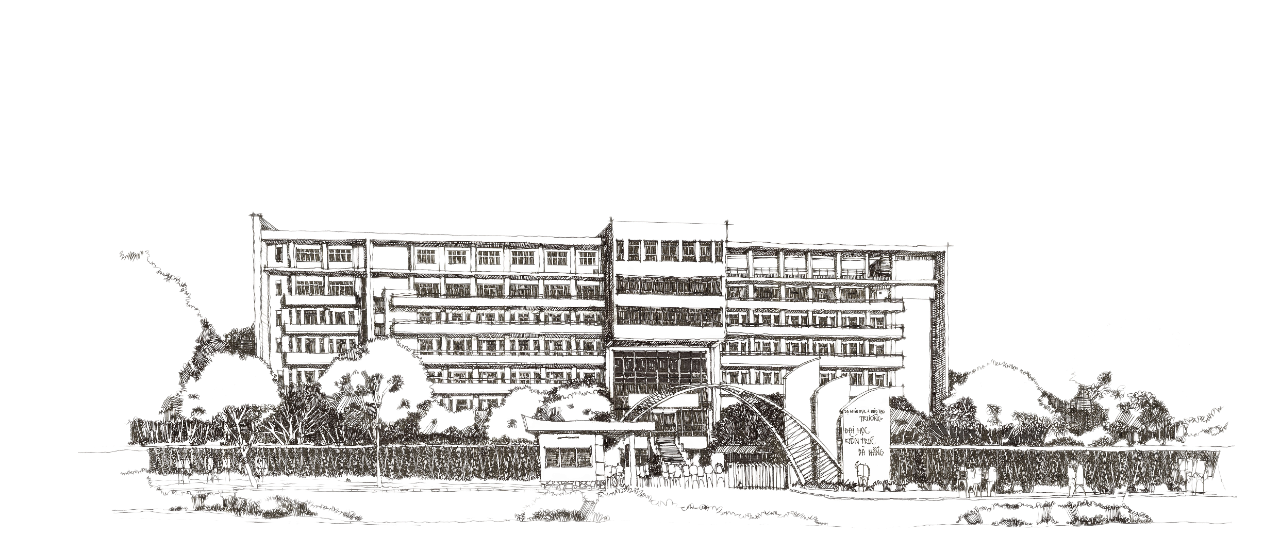
\includegraphics[width=0.5\paperwidth]{dau-campus.png}};
  \node[anchor=north west] at ([xshift=0.6cm, yshift=-0.6cm]current page.north west){
\includegraphics[height=1.0cm]{dau-logo.png}};
  \fill[daumaroon] ([yshift=-4.4cm]current page.north west) rectangle ([yshift=-4.6cm]current page.north east);
  \fill[daugold]   ([yshift=-4.6cm]current page.north west) rectangle ([yshift=-4.72cm]current page.north east);
  \node[anchor=center, text=white, align=center, text width=0.9\paperwidth] at ([yshift=-3.3cm]current page.north){\fontsize{34}{38}\selectfont\bfseries Trân trọng cảm ơn};
  \node[anchor=center, text=white!85, align=center, text width=0.9\paperwidth] at ([yshift=-5.5cm]current page.north){%
    \normalsize TS. Đỗ Phúc Hảo \, $\cdot$ \, Giám đốc Trung tâm CAIRA\\[4pt]
    \small Trường Đại học Kiến trúc Đà Nẵng};
\end{tikzpicture}
\end{frame}}

\end{document}
